\documentclass[12pt]{article}


\usepackage{sbc-template}
\usepackage{graphicx,url}
\usepackage[utf8]{inputenc}
\usepackage[brazil]{babel}

%\usepackage[latin1]{inputenc}
\usepackage{hyperref}
\usepackage{outlines}

\sloppy


\title{Estimativa de Esforço em Projetos de Software com Técnicas\\ de Aprendizado de Máquina}

\author{Carlos A. Bitencourt\inst{1}}

\address{Faculdade de Computação -- Universidade Federal de Mato Grosso do Sul (UFMS)\\79070-900 -- Campo Grande -- MS -- Brazil
  \email{carlos.bitencourt@ufms.br}
}

\begin{document}

\maketitle

\begin{abstract}
  Write after. Write after.Write after.Write after.Write after.Write after.Write after.Write after.Write after.Write after.Write after.Write after.Write after.Write after.Write after.Write after.Write after.Write after.Write after.Write after.Write after.Write after.Write after.Write after.Write after.Write after.Write after.Write
\end{abstract}

\begin{resumo}
  Escrever depois, máximo 10 linhas. Escrever depois,Escrever depois,Escrever depois,Escrever depois,Escrever depois,Escrever depois,Escrever depois,Escrever depois,Escrever depois,Escrever depois,Escrever depois,Escrever depois,Escrever depois,Escrever depois,Escrever depois,Escrever depois,Escrever depois,Escrever depois.

\end{resumo}

\section{Introdução}

No momento atual, é notório a necessidade do desenvolvimento de soluções e serviços digitais confiáveis e seguros. Para alcançar este objetivo, a Engenharia de Software é essencial para a entrega de produtos e serviços com qualidade. Uma das atividades mais importantes é a \textbf{Estimativa de Esforço de Software - EES}. A EES, pode ser aprimorada com o tempo conforme experiência da equipe. Uma vez que a estimativa pode ser aferida por meio de dados históricos, seria possível a implementação de uma solução de \textbf{Aprendizado de Máquina (AM)} para a realização de análise das métricas de um projeto de software? Assim sendo, poder-se-ia aproveitar a base de conhecimento de outras equipes para a predição de estimativas? Reduzindo assim análises equivocadas e tornando cada vez mais preciso as estimativas dos cronogramas dos projetos.

Embora muitas pesquisas tenham sido feitas em EES nos últimos anos, a precisão das estimativas  ainda é uma grande preocupação, tendo em vista, que estimativas imprecisas podem levar a atrasos e aumento de custos em um projeto. Nas últimas décadas, foram propostos vários métodos para estimativa de esforço de software os quais, normalmente, descrevem a estimativa de esforço por meio de fórmulas que consideram parâmetros históricos como por exemplo, experiência da equipe, linguagem de programação dentre outros \cite{asadegravino:2019}.

Assim sendo, o objetivo desse trabalho é realizar uma exploração preliminar da aplicação de ao menos cinco algoritmos de Aprendizagem de Máquina sobre algumas bases de dados públicas contendo informações de EES.

\section{Referencial Teórico} \label{sec:refteorico}

Na fundamentação teórica, para que se possa embasar uma análise adequada, faz-se necessário enumerar e descrever os modelos e técnicas de aprendizado de máquina as serem utilizados nesta pesquisa, bem como uma breve análise das pesquisas sobre estimativa de esforço de software com Aprendizado de Máquina.

\subsection{Aprendizado de Máquina (AM)}

Um dos primeiros exemplos de um sistema de aprendizagem de máquina, foi um programa desenvolvido por Samuel (1959) para jogar damas. Com este programa, foi possível demonstrar como um programa poderia melhorar o seu processamento de dados, sem ser programado. Ou seja, um programa poderia ser treinado para fazer previsões \cite{ieee:2013,samuel:1959}.

Ao longo dos anos, por meio do desenvolvimento de técnicas, métodos e novos algoritmos para o campo da AM foi possível desenvolver uma série de serviços \cite{abadaletal:2020}.

Conceitualmente pode-se delinear a AM com o postulado de Mitchell (1997):
\begin{quote}
  Um programa de computador é dito aprender a partir de uma experiência E com respeito a uma classe de tarefas T e medida de desempenho P, se seu desempenho em tarefas de T, medido por P, melhora a experiência E. \cite[p. 2, tradução nossa]{mitchell:1997}
\end{quote}

Deste modo, por meio de modelos que representam hipóteses, é possível medir o conhecimento aprendido por um processo de indução, que pode ser visto como um processo de busca em que se almeja encontrar a melhor hipótese \cite{stuartnorvig:2013}.

Nas subseções a seguir serão apresentados alguns técnicas, conceitos e algoritmos de aprendizagem de máquina que serão utilizados nesta pesquisa.

\subsubsection{Árvores de Decisão (Decision Tree - DT)}

Uma árvores de decisão toma como entrada um vetor de atributos e retorna uma decisão única. Os valores de entrada e saída podem ser discretos ou contínuos.

\begin{figure}[h]
  \centering
  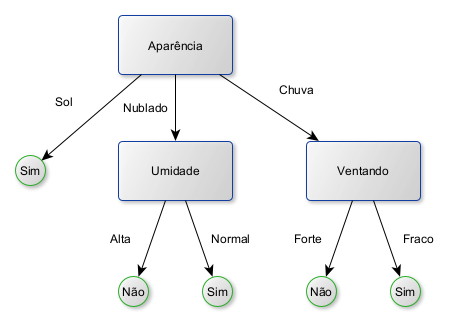
\includegraphics[width=.4\textwidth]{img/fig_arvore_decisao.png}
  \caption{Árvore de Decisão para jogar tênis. Adaptado de Mitchell (1997).}
  \label{fig_arvore_decisao}
\end{figure}

Na Figura~\ref{fig_arvore_decisao}, pode-se observar um exemplo de árvore de decisão, que representa de forma natural ao ser humano os passos para decidir se deve ou não jogar tênis. Cada nó folha da árvore especifica o valor a ser retornado pela função.

Uma forma de medir a importância (ganho de informação) de uma atributo, é por meio do conceito de \textbf{Entropia}, que é a medida de incerteza de uma variável aleatória. Quanto mais informações são necessárias para aprender, maior é a entropia, por outro lado, se não é necessário nenhuma informação a entropia é igual a zero. Dado que a entropia mensura o quão impuro os dados de um coleção estão, pode-se definir o ganho de informação de um atributo A em relação a uma coleção $V$ como:
\begin{equation}
  Ganho(V, A) = Entropia(V) - \sum_{v\in A_k}\frac{|V_v|}{|V|} Entropia(V_v)
\end{equation}
Assim sendo, é possível calcular o Ganho de informação para realização do treinamento. Para dados contínuos, como por exemplo previsão de preços, o algoritmo de árvore de decisão deve encontrar pontos de divisão entre os valores \cite{mitchell:1997,stuartnorvig:2013}.

\subsubsection{Redes Neurais Artificiais (RNA)}

Inspirado no funcionamento do cérebro humano, as Redes Neurais Artificiais são representadas por uma coleção de classificadores lineares conectados cujas propriedades são determinadas pela topologia e pelas propriedades dos ``neurônios'' (Figura~\ref{fig_neuronio}).

\begin{figure}[h]
  \centering
  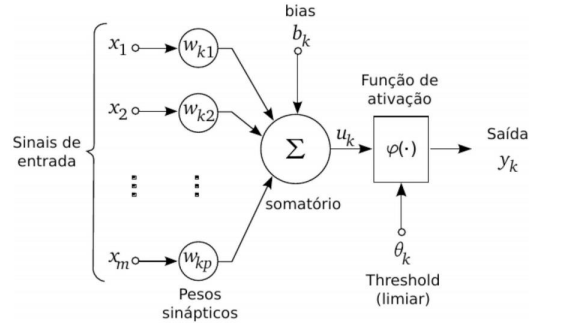
\includegraphics[width=.4\textwidth]{img/fig_neuronio.png}
  \caption{Modelo de Neurônio. Fonte: \cite{haykin:2001}}
  \label{fig_neuronio}
\end{figure}

Um neurônio é uma unidade de processamento de informação onde podemos identificar três elementos básicos. O primeiro é um conjunto de sinais de entradas com \textit{sinapses} caracterizada por pesos ou forças. O segundo, um somador que trata os sinais de entrada. E, por fim uma função de ativação que limita os sinais de saída. Em termos matemáticos pode-se descrever um neurônio $k$ com os sequintes pares de equações:

\begin{equation}
  u_k = \sum_{j = 1}^{m} w_{kj}x_j
\end{equation}
e
\begin{equation}
  y_k = \varphi (u_k + b_k)
\end{equation}
de modo que $x_1, x_2, \ldots, x_n$ são os sinais de entrada; $w_{k1}, w_{k2}, \ldots, w_{km}$ são os pesos sinápticos; $u_k$ a saída dos sinais de entrada; e $y_k$ é o sinal de saída.

É possível organizar a topologia de uma rede neural em diversas camadas, com diferentes número de unidades por camada, aumentando a capacidade da rede de aprender \cite{haykin:2001}.

\subsubsection{K-Vizinhos Mais Próximos (\textbf{K-Nearest Neighbors - KNN})}

Algoritmos baseados em instâncias baseiam o seu aprendizado no armazenamento dos dados de treinamento para utilização na classificação de uma entrada nova. Um dos algoritmos mais utilizados nesta abordagem é o \textbf{KNN}.

Os vizinhos mais próximos podem ser calculados pela \textbf{distância euclidiana}. Dado uma instância $x$ descrita pelo vetor $[a_1(x), a_2(x), \ldots a_n(x)]$, onde $a_k$ é o $k$-ésimo atributo da instância x, então a distância de $x_i$ e $x_j$ é definida:
\begin{equation}
  d(x_i, x_j) = \sqrt{\sum_{k = 1}^{n} (a_k(x_i) + a_k(x_j))^2 }
\end{equation}

Para classificar, primeiro encontre os $k$ vizinhos mais próximos e realize um processo de contagem. A classe majoritária será atribuída ao novo objeto. Para evitar empates, recomenda-se sempre escolher um número ímpar para $k$. Para classes contínuas, pode-se tirar a média ou mediana de $k$ vizinhos \cite{mitchell:1997,stuartnorvig:2013}.

\subsubsection{Máquinas de Vetor de Suporte (Support Vector Machine - SVM)}
A \textbf{Máquina de Vetor de Suporte (SVM)} contém três propriedades relevantes. A primeira, diz respeito a capacidade de construir um \textbf{separador de margem máxima} que contribui na generalização. A segunda, é a capacidade de, além de tratar dados lineares, incorporar os dados em um espaço de dimensão superior. Terceiro, apesar de ser um método não paramétrico, na prática, acabam mantendo apenas uma fração do número de exemplos. A idéia é considerar alguns exemplos mais importantes que os outros o que pode levar a uma generalização melhor.

\begin{figure}[h]
  \centering
  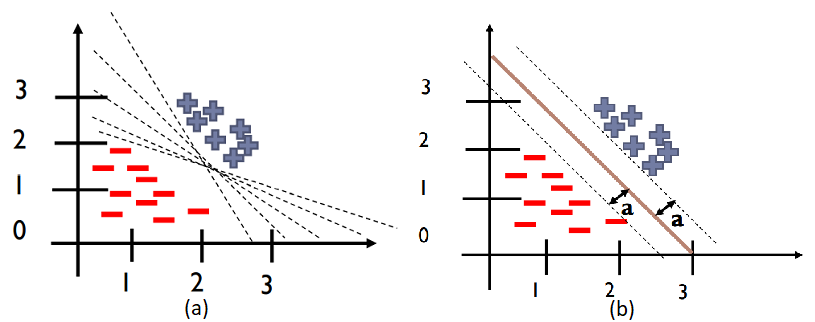
\includegraphics[width=.6\textwidth]{img/fig_svm.png}
  \caption{Máquina de Vetor de Suporte. (a) Duas classes vários separadores lineares candidatos. (b) O separador de margem máxima ao centro. Adaptado de \cite{bruno:2020}}
  \label{fig_svm}
\end{figure}

Na Figura~\ref{fig_svm}, pode-se observar em (a) várias possibilidades de separação, enquanto em (b) busca-se o separador médio mais distantes das classes, chama-se o separador de \textbf{margem máxima}, dessa forma pode-se minimizar a perda de generalização \cite{stuartnorvig:2013}.

\subsubsection{Floresta Aleatória (Random Florest - RF)}

O Algoritmo de Floresta Aleatória consiste em um classificador cuja topologia é uma coleção de classificadores estruturados em árvores.

\begin{figure}[h]
  \centering
  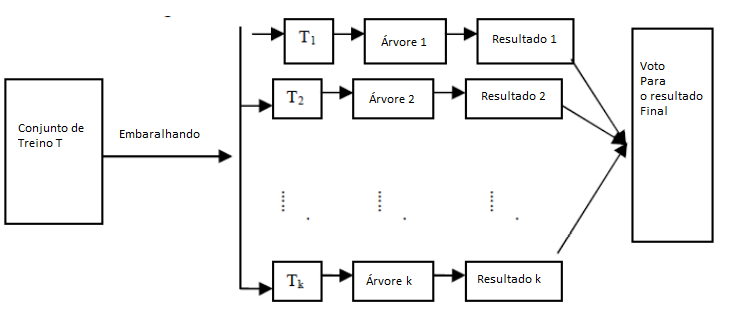
\includegraphics[width=.4\textwidth]{img/fig_random_forest.png}
  \caption{Modelo de Floresta Aleatória. Adaptado de \cite{liuetal:2012}}
  \label{fig_random_forest}
\end{figure}

Como pode-se observar na Figura \ref{fig_random_forest}, cada árvore recebe um conjunto de treinamento aleatório, que após os dados toma uma decisão representada pela equação \ref{eq_random_forest}:

\begin{equation}
  H(x) = arg \max_Y \sum_{i = 1}^{k} I (h_i(x) = Y)
  \label{eq_random_forest}
\end{equation}
onde $H(x)$ é uma combinação do modelo de classificação, $h_i$ é a decisão de uma das árvores, $Y$ é a variável de saída. Cada árvore tem direito a um voto para selecionar o melhor resultado de classificação \cite{liuetal:2012}.


\subsection{Estimativa de Esforço de Software e Aprendizagem de Máquina}

Muitas pesquisas tem sido feitas na área de estimativas de esforço de softwares nos últimos anos. No entanto, a precisão das estimativas de esforço de software ainda é uma grande preocupação, tendo em vista, que estimativas imprecisas podem levar a atrasos e aumento de custos em um projeto. Nas últimas décadas, foram propostos vários métodos para estimativa de esforço de software os quais, normalmente, descrevem a estimativa de esforço por meio de fórmulas que consideram parâmetros históricos como por exemplo, experiência da equipe, linguagem de programação dentre outros \cite{asadegravino:2019}.

Nas ultimas três décadas os estudos que aplicam o AM na estimativa de software foi ampliado motivado pela ampla margem de erro nos métodos tradicionais de estimativa e pela melhoria contínua dos algoritmos de aprendizado de máquina \cite{banimustafa:2018}.

Vários algoritmos foram utilizados para estimar esforço, custo e tempo de desenvolvimento de software. A maioria dessas técnicas foram aplicadas a dados públicos. Árvore de Decisão, Florestas de Árvores de Decisão em \cite{nassifetal:2013}, o uso de programação genética foi relatado em \cite{chavoyaetal:2012}. Uso de Redes Neurais Artificiais foram usadas para prever o esforço e foram comparadas com a estimativa do modelo COMOMO \cite{trontoetal:2007, bhatiaattri:2015} dentre muitos outros trabalhos.

Ali e Gravino (2019) por meio de uma revisão sistemática da literatura sobre estimativa de eforço de software baseado em aprendizam de máquina, resgataram a análise sistemática de \cite{wen:2012} e complementaram com os próximos anos. Nesta análise, eles reponderam questões como quais as bases de dados mais utilizadas nas pesquisas? Quais os algoritmos quais obtiveram o maior desempenho? Quais as métricas mais utilizadas? Dentre os estudos avaliados, as três técnicas mais utilizadas foram respectivamente Redes Neurais Artificiais, Máquinas de Vetores de Suporte e Redes Bayseanas. A técnica K-Vizinhos Mais Próximos em quinto, Árvores de Decisão em sexto e por fim, Floresta Aletória em oitava posição. Dentre as bases de dados mais usadas nos estudos, as três primeiras foram a NASA, COCOMO e ISBSG respectivamente.

Em relação as métricas, Magnitude Média do Erro Relativo (Mean Magnitude of Relative Error - MMRE) e Porcentagem de Previsões de 25 por cento (Percentage of Predictions - Pred(25)) foram amplamente usadas sendo que o Erro Absoluto Médio (Mean Absolute Error - MAE) ficou em quarto mais utilizado.

\section{Metodologia}

Para realização da pesquisa, foram selecionadas cinco bases de dados disponíveis publicamente, todas  relacionadas a Estimativas de Esforço de Software (Tabela \ref{tab_bases}): Cocomo81 (D1), Cocomonasa (D2), Desharnais (D3), Nasanumeric (D4) e Seera (D5) \cite{promise:2005, nasanumeric:2014, seera:2020}.

\begin{table}[h!]
  \begin{center}
    \caption{Base de Dados}
    \label{tab_bases}
    \begin{tabular}{r|c|c|c|c}
      \textbf{ID}      & \textbf{Nº Atr.} & \textbf{Nº Atr.} & \textbf{Nº Linhas} & \textbf{Nº Linhas} \\
      \textbf{}        & \textbf{Inicial} & \textbf{Final}   & \textbf{ Inicial}  & \textbf{Final}     \\
      \hline
      Cocomo81 (D1)    & 17               & 17               & 63                 & 63                 \\
      Cocomonasa (D2)  & 17               & 17               & 60                 & 60                 \\
      Desharnais (D3)  & 12               & 17               & 81                 & 60                 \\
      Nasanumeric (D4) & 24               & 41               & 93                 & 93                 \\
      Seera (D5)       & 76               & 33               & 120                & 111                \\
    \end{tabular}
  \end{center}
\end{table}

As bases de dados D1, D2, D3 e D4 possuem atributos semelhantes relacionados a técnica de Estimativa de Software COCOMO \cite{boehm:1981}. Este modelo, estima o esforço de desenvolvimento de software em relação a homem-mês considerando o tamanho do código (LOC) ou Pontos por função \cite{banimustafa:2018}. A fórmula geral:

\begin{equation}
  Effort = A S^b
\end{equation}

Sendo $A$ um parâmetro de produtividade, $b$ um parâmetro escalável de economia e $S$ linhas por código (LOC) ou Pontos por função \cite{shepperd:1997}.

Deste modo, ``Effort'' representa o atributo Classe das Bases de Dados. A base de dados D5, possui dados mais recentes e completos contendo 76 atributos inicialmente, muito mais que as demais bases, 24 (D4), 12 (D3) e 17 (D1, D2) (Tabela \ref{tab_bases}).

Para tratamento dos dados, optou-se por excluir linhas cujos os dados fossem nulos ou vazios. Deste modo, após a identificação e exclusão destas linhas, não houve alteração nas bases D1, D2 e D3, foram removidas 19 linhas da base D4 e 11 linhas da base D5. Em relação aos atributos, foi necessário o ajuste de atributos textuais em numéricos nas bases D2 e D4, ajustes em atributos categóricos nas bases D3 (``language''), D4 (``cat2'') e D5 (``Programming language used''), resultando na alteração do número dos atributos finais como pode ser observado na Tabela \ref{tab_bases}. Além disso, foram removidos alguns atributos descritivos como ano de projeto e identificadores. Para a base D5, foram removidos vários atributos cujo valor compunha outro atributo presente, ou seja, dados derivados, mantendo-se atributos considerados relavantes e semelhantes as demais bases.

Após, as bases de dados foram submetidas a transformação na mesma ordem de grandeza por meio do método \textit{z-score}.

\subsection{Ajustes e Treinamento dos Classificadores / Regressores}

Foram selecionados cinco Algoritmos para análise de performance (Tabela \ref{tab_algoritmos}): Árvore de Decisão (DT), Redes Neurais Artificiais (Perceptron Multi-camadas - MLP), K-Vizinhos Mais Próximos (KNN), Máquinas de Vetor de Suporte (SVM) e Floresta Aleatório (RF).

Para implementação e execução da análise foi utilizado a biblioteca \textit{Scikit-learn} \cite{scikitlearn:2011} com a linguagem de programação \textit{Python}.

\begin{table}[h!]
  \begin{center}
    \caption{Algoritmos e componentes \textit{Scikit-learn}}
    \label{tab_algoritmos}
    \begin{tabular}{l|l}
      \textbf{Algoritmos} & \textbf{Componentes}  \\
      \hline
      DT                  & DecisionTreeRegressor \\
      MLP                 & MLPRegressor          \\
      KNN                 & KNeighborsRegressor   \\
      SVM                 & SVM                   \\
      RF                  & RandomForestRegressor \\
    \end{tabular}
  \end{center}
\end{table}

Para o treinamento optou-se por usar a validação cruzada de \textit{3-folds} e a  \textbf{Média do Erro Absoluto (MAE)} como métrica de avaliação do melhor modelo. Para cada algoritmo buscou-se a melhor configuração de parâmetros retornada pelo \textit{GridSearchCV} por meio dos seguintes passos:

\begin{outline}[enumerate]
  \1 Para uma base e algoritmo, roda o \textit{GridSearchCV} com opções de variáveis escolhidas iniciais.
  \1 Caso, o melhor parâmetro para uma determinada variável pertence a fronteira.
    \2 Ajusta a opções de parâmetros extendendo a fronteira. Ex: opções iniciais [2,4,8], melhor opção [2] então novas opções [0, 2, 4].
  \1 Volta ao passo 1, até que os melhores parâmetros não pertençam a fronteira de opções.
 \end{outline}

 Deste modo, os resultados serão apresentados na seção a seguir.

\section{Análise e Discussão}

Os melhores parâmetros encontrados para os 5 algoritmos propostos considerando a base de dados são apresentados na Tabela \ref{tab_parametros}.

\begin{table}[h!]
  \begin{center}
    \caption{Algoritmos, base de dados, melhores parâmetros}
    \label{tab_parametros}
    \begin{tabular}{r|c|l}
      \textbf{Algoritmos} & \textbf{Base de Dados} & \textbf{ Mellhores Parâmetros} \\
      \hline
      DT                  & D1 & a  \\
      MLP                 & D1 & a  \\
      KNN                 & D1 & a  \\
      SVM                 & D1 & a  \\
      RF                  & D1 & a  \\
      DT                  & D2 & a  \\
      MLP                 & D2 & a  \\
      KNN                 & D2 & a  \\
      SVM                 & D2 & a  \\
      RF                  & D2 & a  \\
      DT                  & D3 & a  \\
      MLP                 & D3 & a  \\
      KNN                 & D3 & a  \\
      SVM                 & D3 & a  \\
      RF                  & D3 & a  \\
      DT                  & D4 & a  \\
      MLP                 & D4 & a  \\
      KNN                 & D4 & a  \\
      SVM                 & D4 & a  \\
      RF                  & D4 & a  \\
      DT                  & D5 & a  \\
      MLP                 & D5 & a  \\
      KNN                 & D5 & a  \\
      SVM                 & D5 & a  \\
      RF                  & D5 & a  \\
    \end{tabular}
  \end{center}
\end{table}

Para os melhores parâmetros, os algoritmos alcançaram os desempenhos relacionados na Tabela \ref{tab_desempenho}.

\begin{table}[h!]
  \begin{center}
    \caption{Algoritmos e Desempenho em Erro Absoluto Médio (MAE) }
    \label{tab_desempenho}
    \begin{tabular}{l|c|c|c|c|c}
      \textbf{Algoritmos} & \textbf{D1} & \textbf{D2} & \textbf{D3} & \textbf{D4} & \textbf{D5} \\
      DT                  & 1           & 1           & 1           & 1           & 1           \\
      MLP                 & 1           & 1           & 1           & 1           & 1           \\
      KNN                 & 1           & 1           & 1           & 1           & 1           \\
      SVM                 & 1           & 1           & 1           & 1           & 1           \\
      RF                  & 1           & 1           & 1           & 1           & 1           \\
    \end{tabular}
  \end{center}
\end{table}



\section{Conclusão}\label{sec:figs}




\bibliographystyle{sbc}
\bibliography{sbc-template}

\end{document}
